\chapter{Results on Surrogate Model Performance}
Please choose a more expressive title for this chapter. If it makes sense for your work you can also have multiple chapters presenting your results.

\section{Training Effectivity}

\begin{figure}
    \centering
    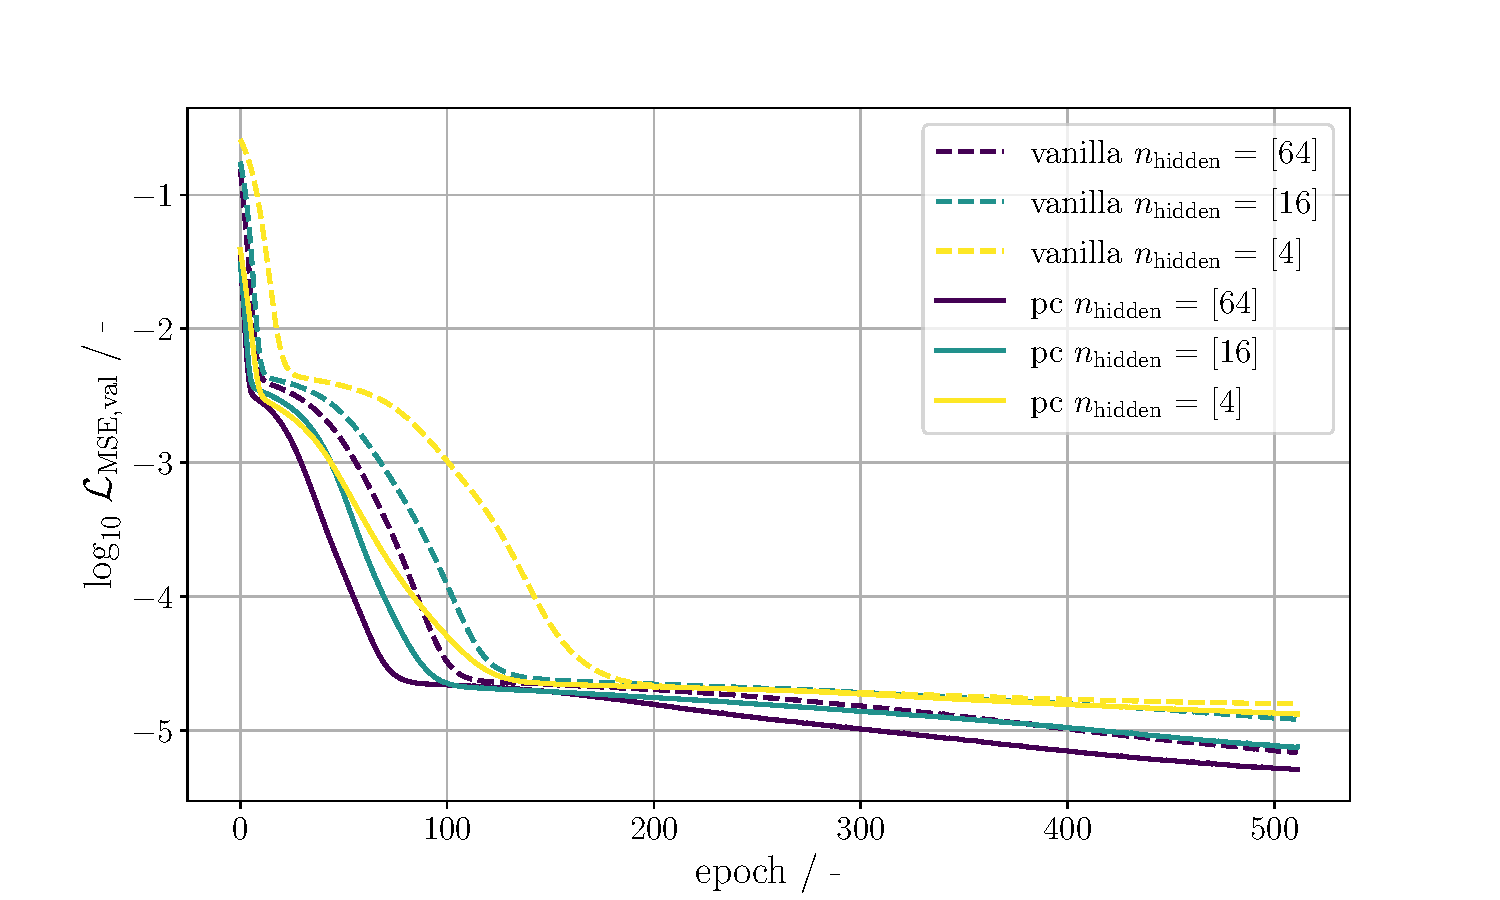
\includegraphics[width=1\textwidth]{Figures/Results/001_val_loss.pdf}
    \caption[Validation loss of vanilla NARX vs physics-constrained NARX]{The validation loss calculated as MSE $\mathcal{L}_\mathrm{MSE, val}$
    during the training of the vanilla NARX (dashed line) and the physics-constrained NARX (solid line). The three data rows each indicate
    \emph{one hidden layer} with $64, 16$ and $4$ hidden neurons respectively. The physics-constrained NARX converges visibly faster
    than the vanilla NARX.}
    \label{intro:fig:01_data}
\end{figure}
